{\textbf{1. 概念描述}}

{{分块查找又称为索引顺序查找},其数据结构可以简单描述为:分块查找把线性表分成若干块,{每一块中元素的存储顺序是任意的,但是块与块之间必须按照关键字大小有序排列},即前一块中的最大关键字要小于后一块中的最小关键字。对顺序表进行分块查找需要额外建立一个索引表,表中的每一项对应线性表中的一块。}{索引表的定义如下:}

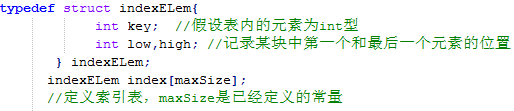
\includegraphics[width=3.70833in,height=0.80208in]{png-jpeg-pics/7B6353AA0580E0C833864C13ECA0965F.png}

{\textbf{~2. 算法描述}}

{分块查找算法非常简单,可以分为两步进行,{首先确定待查找的元素属于哪一块,然后在块内精确查找该元素}。由于索引表是递增有序的,因此第一步采用二分查找。块内元素一般个数较少,因此第二步采用顺序查找即可。}

分块查找实际上进行{\textbf{两次查找}},{整个算法的平均查找长度是两次查找的平均查找的平均查找长度之和},即二分查找平均查找长度+顺序查找平均查找长度。

~ ~ ~ ~
